% ==============================================================================
% SECTION 2: NETWORK ARCHITECTURE & TOPOLOGY DESIGN (STEP 1)
% ==============================================================================
\section{Network Architecture \& Topology Design (Step 1)}

\subsection{Multi-Campus Hierarchical Architecture}
The redesigned TVI enterprise infrastructure spans \textbf{10 Cisco IOS network nodes} organized into three corporate Autonomous Systems (\texttt{AS 65001}, \texttt{AS 65002}, \texttt{AS 65003}) interconnected across an ISP provider cloud (\texttt{AS 65000}). To align hardware utilization with campus scale while maintaining strict fault-domain isolation, two complementary campus switching patterns are deployed:

\begin{itemize}[leftmargin=1.5em, itemsep=3pt]
    \item \textbf{TP.HCM Headquarters (Three-Tier / Dual-Distribution Architecture, \texttt{AS 65001}):} Separates the WAN routing boundary (\texttt{HCMC-EDGE-RTR01}), redundant Layer~3 Distribution switching (\texttt{HCMC-DIST-SW01} and \texttt{HCMC-DIST-SW02}), and Layer~2 Access switching (\texttt{HCMC-CORE-SW01}). Layer~2 loops are strictly contained beneath the distribution switches using LACP \texttt{Port-channel 1} and Rapid-PVST+, while routed Layer~3 uplinks (\texttt{/30} point-to-point links) eliminate broadcast propagation toward the WAN edge.
    \item \textbf{Hanoi R\&D (\texttt{AS 65002}) \& Da Nang Logistics (\texttt{AS 65003}) (Collapsed Branch Edge):} Each branch utilizes a dedicated Cisco edge router (\texttt{HANOI-RND-RTR01}, \texttt{DANANG-LOG-RTR01}) performing Router-on-a-Stick (\texttt{802.1Q} sub-interfaces) over a trusted trunk to regional Layer~2 switches (\texttt{HANOI-RND-SW01/SW02} linked via LACP \texttt{Po1}, and \texttt{DANANG-LOG-SW01}).
\end{itemize}

\subsection{Layer 2/Layer 3 Boundaries, WAN Demarcation \& Trust Zones}
A disciplined enterprise topology must establish unambiguous boundaries between Layer~2 switching domains, Layer~3 routing planes, service-provider demarcation points, and security trust zones:

\begin{enumerate}[leftmargin=1.5em, itemsep=3pt]
    \item \textbf{WAN Demarcation Points (CE $\leftrightarrow$ PE):} Located cleanly at \texttt{GigabitEthernet0/0} on all three campus edge routers (\texttt{HCMC-EDGE-RTR01}, \texttt{HANOI-RND-RTR01}, \texttt{DANANG-LOG-RTR01}) facing \texttt{ISP-CORE-RTR01} (\texttt{AS 65000}). Inside the demarcation line, TVI retains full control over PAT/NAT Overload, outbound LLQ QoS queuing, IPsec encryption endpoints, and BGP prefix filtering.
    \item \textbf{Underlay vs. Overlay Separation:} Physical WAN \texttt{/30} links (\texttt{203.0.113.0/30}, \texttt{.4/30}, \texttt{.8/30}) form the public eBGP underlay reaching the simulated public DNS server (\texttt{Loopback0: 8.8.8.8/32}). Encrypted \textbf{GRE over IPsec VPN} tunnels (\texttt{Tunnel12} and \texttt{Tunnel13}) ride above this underlay to establish private point-to-point Layer~3 adjacencies running \textbf{OSPFv2/OSPFv3 Area~0}.
    \item \textbf{Security Trust Zones:}
    \begin{itemize}[leftmargin=1.4em, itemsep=2pt]
        \item \emph{Restricted Trust Zone (\texttt{VLAN 10 - EXEC\_FINANCE}):} Hosts executive workstations and TVI's centralized DHCP/DNS/NTP enterprise server (\texttt{10.10.10.50}).
        \item \emph{Corporate Production Zones (\texttt{VLAN 20 - RND\_ENGINEERING}, \texttt{VLAN 30 - LOGISTICS\_OPS}):} Support HQ/Hanoi engineers and Da Nang warehouse IoT sensors, protected by Port Security, DHCP Snooping, and DAI.
        \item \emph{Out-of-Band Management Zone (\texttt{VLAN 99 - MANAGEMENT}):} Isolates SSHv2 management interfaces (\texttt{192.168.1.10}, \texttt{192.168.2.10--11}, \texttt{192.168.3.10}) and the Python Netmiko automation controller from user broadcast traffic.
        \item \emph{Untrusted Isolation Zone (\texttt{VLAN 50 - GUEST\_WIFI}):} Strictly isolated at \texttt{HANOI-RND-RTR01 Gi0/1.50} via an inbound Extended ACL permitting public Internet access while denying all RFC~1918 corporate destinations.
        \item \emph{Blackhole Quarantine (\texttt{VLAN 999 - BLACKHOLE}):} All unused switch ports across all three campuses are statically assigned to \texttt{VLAN 999} and administratively shut down.
    \end{itemize}
\end{enumerate}

\subsection{Comprehensive Logical \& Physical Network Topology Diagram}
Figure~\ref{fig:tvi_topology} presents the complete Draw.io logical and physical topology diagram, detailing all 10 network devices, interface IDs, IPv4/IPv6 boundaries, HSRP virtual gateways, LACP trunks, WAN demarcation points, and IPsec overlay tunnels.

\begin{figure}[H]
    \centering
    \setlength{\fboxsep}{2pt}
    \setlength{\fboxrule}{0.6pt}
    \fcolorbox{BorderGray}{white}{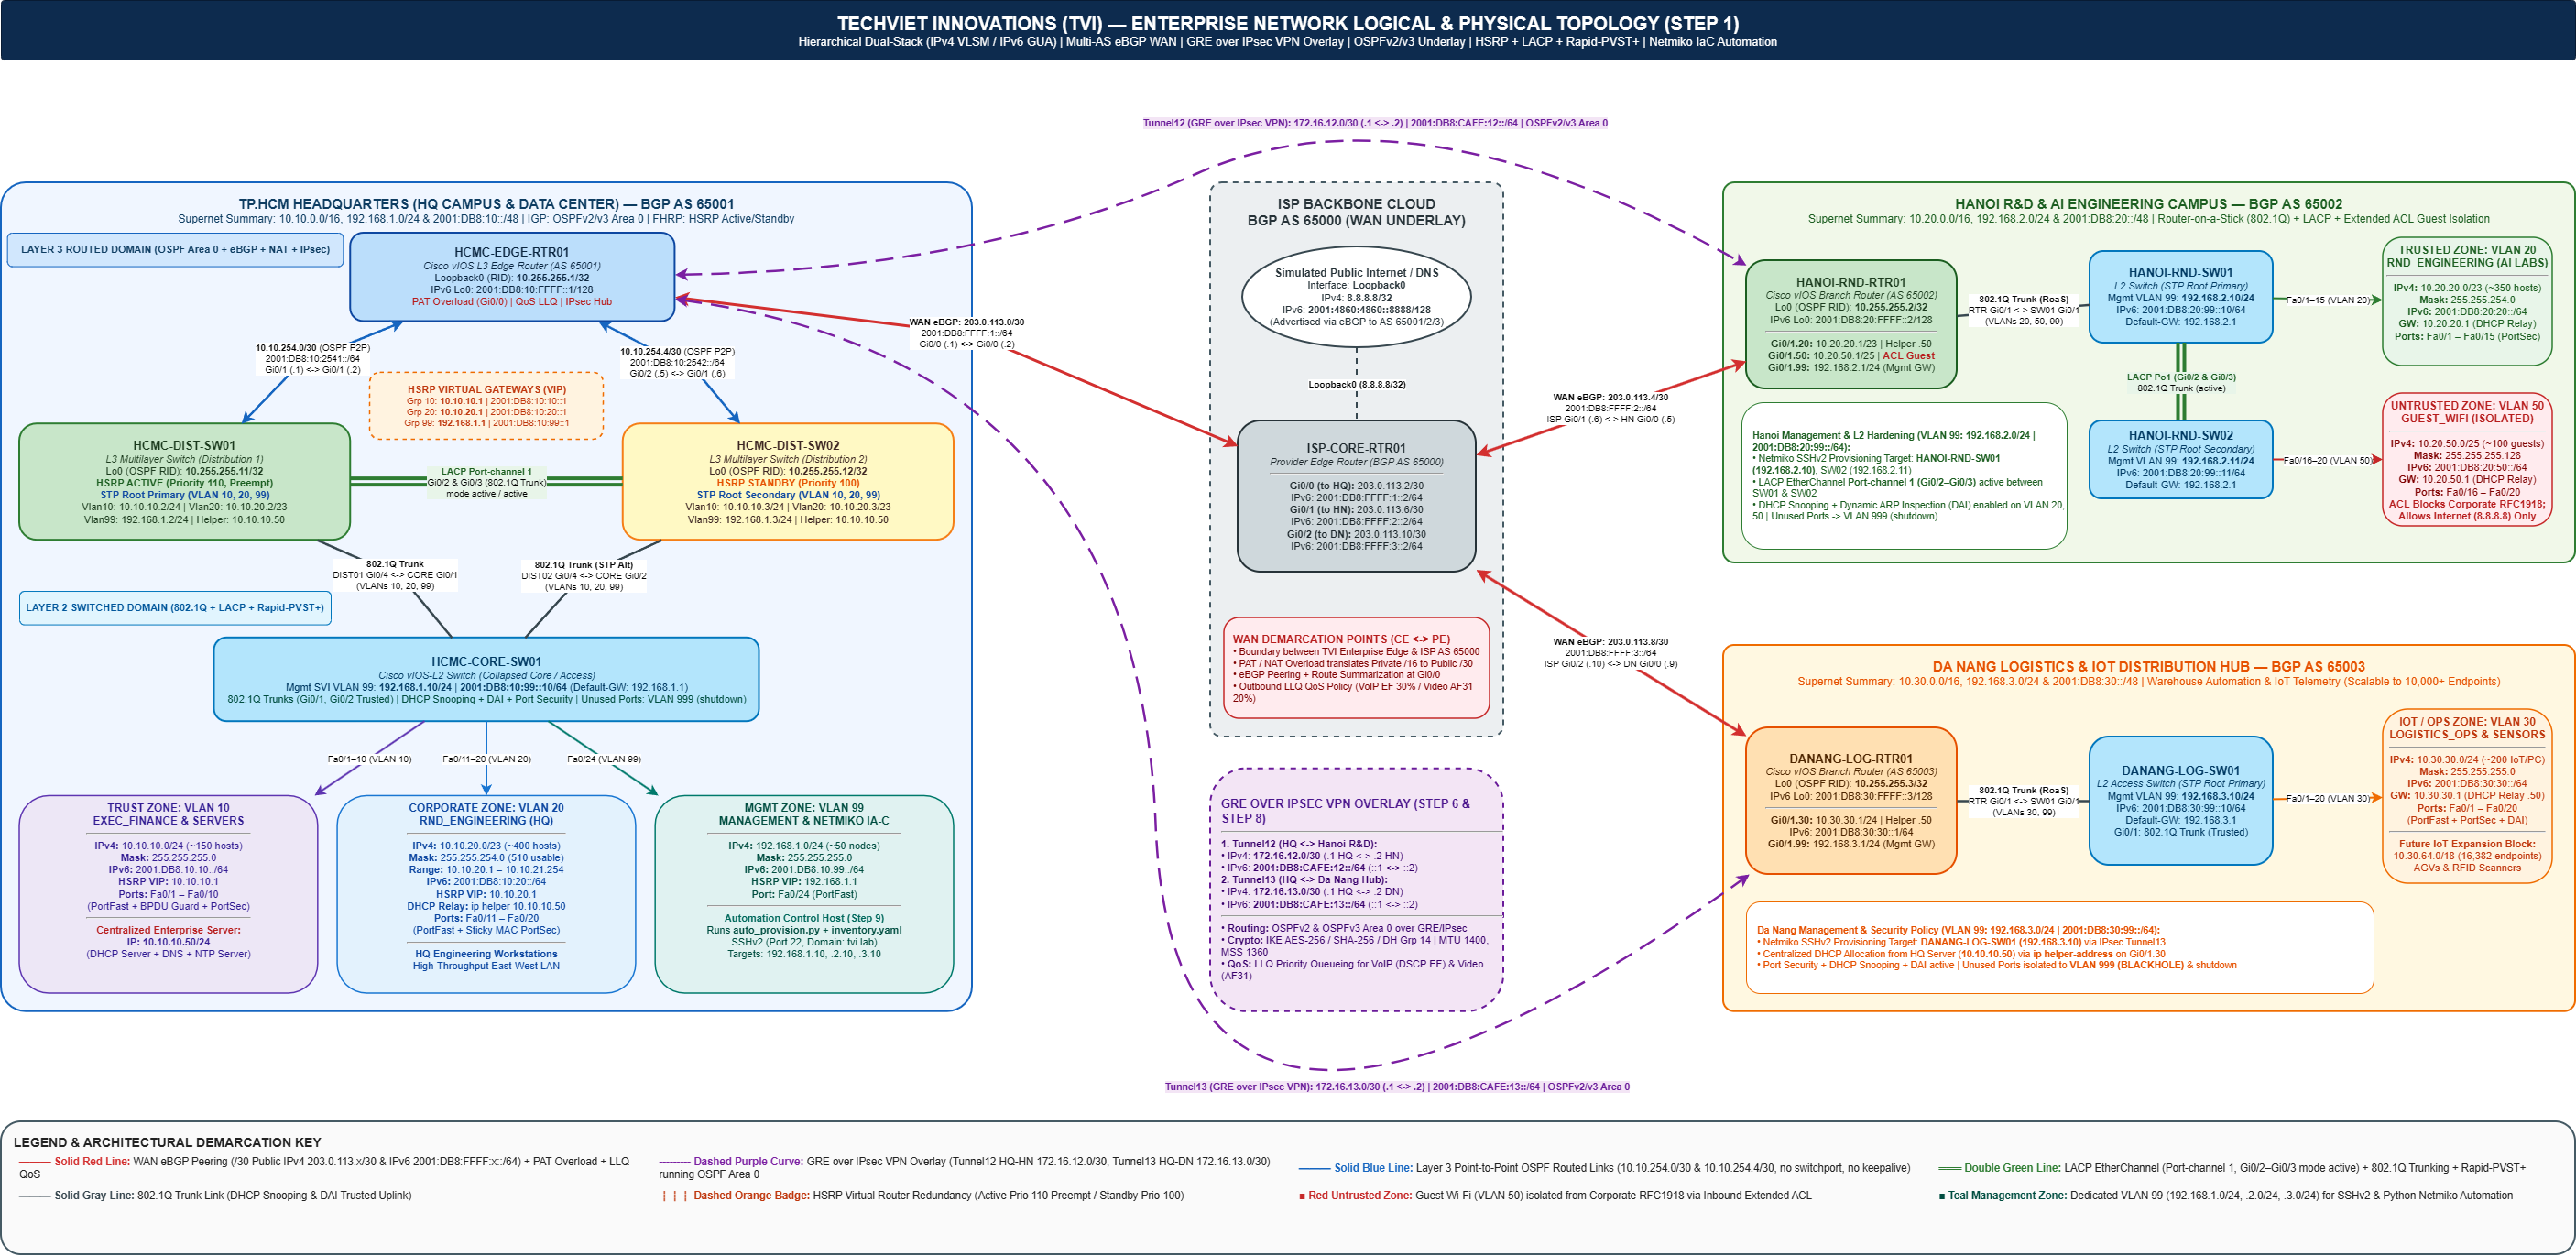
\includegraphics[width=0.98\textwidth]{TVI_Network_Topology.png}}
    \caption{Complete Logical and Physical Enterprise Topology for TechViet Innovations (TVI) across Ho Chi Minh City HQ, Hanoi R\&D, Da Nang Logistics, and ISP Cloud.}
    \label{fig:tvi_topology}
\end{figure}

\subsection{Port-by-Port Interface Mapping Contract}
To guarantee zero interface mismatch during parallel configuration across the engineering team, Table~\ref{tab:port_mapping_hq} and Table~\ref{tab:port_mapping_branches} specify the immutable port-by-port wiring and protocol assignment for all 10 network devices.

\begin{table}[H]
\centering
\caption{Port-by-Port Interface Wiring and Protocol Contract: ISP Backbone \& TP.HCM HQ.}
\label{tab:port_mapping_hq}
\scriptsize
\setlength{\tabcolsep}{4pt}
\begin{tabularx}{\textwidth}{|p{2.4cm}|p{1.35cm}|p{2.7cm}|p{3.2cm}|X|}
\hline
\textbf{Device (AS / Role)} & \textbf{Interface} & \textbf{Connected Peer / Scope} & \textbf{Mode / Protocol} & \textbf{IPv4 \& IPv6 Dual-Stack Address} \\
\hline
\multirow{4}{2.4cm}{\textbf{ISP-CORE-RTR01}\\(\texttt{AS 65000}, PE)}
 & \texttt{Gi0/0} & \texttt{HCMC-EDGE-RTR01 Gi0/0} & L3 WAN (eBGP) & \texttt{203.0.113.2/30} \textbar\ \texttt{2001:DB8:FFFF:1::2/64} \\
 & \texttt{Gi0/1} & \texttt{HANOI-RND-RTR01 Gi0/0} & L3 WAN (eBGP) & \texttt{203.0.113.6/30} \textbar\ \texttt{2001:DB8:FFFF:2::2/64} \\
 & \texttt{Gi0/2} & \texttt{DANANG-LOG-RTR01 Gi0/0} & L3 WAN (eBGP) & \texttt{203.0.113.10/30} \textbar\ \texttt{2001:DB8:FFFF:3::2/64} \\
 & \texttt{Loopback0} & Simulated Internet DNS & Loopback (BGP Adv.) & \texttt{8.8.8.8/32} \textbar\ \texttt{2001:4860:4860::8888/128} \\
\hline
\multirow{6}{2.4cm}{\textbf{HCMC-EDGE-RTR01}\\(\texttt{AS 65001}, HQ Edge)}
 & \texttt{Gi0/0} & \texttt{ISP-CORE-RTR01 Gi0/0} & \texttt{nat outside}, eBGP, QoS & \texttt{203.0.113.1/30} \textbar\ \texttt{2001:DB8:FFFF:1::1/64} \\
 & \texttt{Gi0/1} & \texttt{HCMC-DIST-SW01 Gi0/1} & \texttt{nat inside}, OSPF Area 0 & \texttt{10.10.254.1/30} \textbar\ \texttt{2001:DB8:10:2541::1/64} \\
 & \texttt{Gi0/2} & \texttt{HCMC-DIST-SW02 Gi0/1} & \texttt{nat inside}, OSPF Area 0 & \texttt{10.10.254.5/30} \textbar\ \texttt{2001:DB8:10:2542::1/64} \\
 & \texttt{Loopback0} & OSPF Router-ID & Loopback (Area 0) & \texttt{10.255.255.1/32} \textbar\ \texttt{2001:DB8:10:FFFF::1/128} \\
 & \texttt{Tunnel12} & \texttt{HANOI-RND-RTR01 Tun12} & GRE/IPsec + OSPF + QoS & \texttt{172.16.12.1/30} \textbar\ \texttt{2001:DB8:CAFE:12::1/64} \\
 & \texttt{Tunnel13} & \texttt{DANANG-LOG-RTR01 Tun13} & GRE/IPsec + OSPF + QoS & \texttt{172.16.13.1/30} \textbar\ \texttt{2001:DB8:CAFE:13::1/64} \\
\hline
\multirow{8}{2.4cm}{\textbf{HCMC-DIST-SW01}\\(HSRP Active 110, STP Root Pri.)}
 & \texttt{Gi0/1} & \texttt{HCMC-EDGE-RTR01 Gi0/1} & L3 (\texttt{no switchport}) & \texttt{10.10.254.2/30} \textbar\ \texttt{2001:DB8:10:2541::2/64} \\
 & \texttt{Gi0/2--3} & \texttt{HCMC-DIST-SW02 Gi0/2--3} & LACP \texttt{Po1} (802.1Q) & \emph{Layer 2 Trunk (Mode Active)} \\
 & \texttt{Gi1/0} & \texttt{HCMC-CORE-SW01 Gi0/1} & 802.1Q Trunk (Pri.) & \emph{Layer 2 Trunk (VLANs 10, 20, 99)} \\
 & \texttt{Gi0/0, 1/1--3/3} & Unused Switch Ports & \texttt{VLAN 999} (\texttt{shutdown}) & \emph{Blackhole Quarantine (Disabled)} \\
 & \texttt{Vlan 10} & Executive / Server SVI & HSRP Grp 10 (VIP \texttt{.1}) & \texttt{10.10.10.2/24} \textbar\ \texttt{2001:DB8:10:10::2/64} \\
 & \texttt{Vlan 20} & R\&D SVI & HSRP Grp 20 + Helper \texttt{.50} & \texttt{10.10.20.2/23} \textbar\ \texttt{2001:DB8:10:20::2/64} \\
 & \texttt{Vlan 99} & Management SVI & HSRP Grp 99 (VIP \texttt{.1}) & \texttt{192.168.1.2/24} \textbar\ \texttt{2001:DB8:10:99::2/64} \\
 & \texttt{Loopback0} & OSPF Router-ID & Loopback (Area 0) & \texttt{10.255.255.11/32} \textbar\ \texttt{2001:DB8:10:FFFF::11/128} \\
\hline
\multirow{8}{2.4cm}{\textbf{HCMC-DIST-SW02}\\(HSRP Standby 100, STP Root Sec.)}
 & \texttt{Gi0/1} & \texttt{HCMC-EDGE-RTR01 Gi0/2} & L3 (\texttt{no switchport}) & \texttt{10.10.254.6/30} \textbar\ \texttt{2001:DB8:10:2542::2/64} \\
 & \texttt{Gi0/2--3} & \texttt{HCMC-DIST-SW01 Gi0/2--3} & LACP \texttt{Po1} (802.1Q) & \emph{Layer 2 Trunk (Mode Active)} \\
 & \texttt{Gi1/0} & \texttt{HCMC-CORE-SW01 Gi0/2} & 802.1Q Trunk (Alt.) & \emph{Layer 2 Trunk (VLANs 10, 20, 99)} \\
 & \texttt{Gi0/0, 1/1--3/3} & Unused Switch Ports & \texttt{VLAN 999} (\texttt{shutdown}) & \emph{Blackhole Quarantine (Disabled)} \\
 & \texttt{Vlan 10} & Executive / Server SVI & HSRP Grp 10 (Prio 100) & \texttt{10.10.10.3/24} \textbar\ \texttt{2001:DB8:10:10::3/64} \\
 & \texttt{Vlan 20} & R\&D SVI & HSRP Grp 20 + Helper \texttt{.50} & \texttt{10.10.20.3/23} \textbar\ \texttt{2001:DB8:10:20::3/64} \\
 & \texttt{Vlan 99} & Management SVI & HSRP Grp 99 (Prio 100) & \texttt{192.168.1.3/24} \textbar\ \texttt{2001:DB8:10:99::3/64} \\
 & \texttt{Loopback0} & OSPF Router-ID & Loopback (Area 0) & \texttt{10.255.255.12/32} \textbar\ \texttt{2001:DB8:10:FFFF::12/128} \\
\hline
\multirow{7}{2.4cm}{\textbf{HCMC-CORE-SW01}\\(HQ L2 Access, 16-port vIOS-L2)}
 & \texttt{Gi0/1--2} & \texttt{DIST-SW01/02 Gi1/0} & 802.1Q Trunk (Trusted) & \emph{DHCP Snooping \& DAI Trusted} \\
 & \texttt{Gi0/0} & DHCP/DNS/NTP Server & Access \texttt{VLAN 10} & \emph{PortFast (Server \texttt{10.10.10.50})} \\
 & \texttt{Gi0/3} & Executive/Finance PCs & Access \texttt{VLAN 10} & \emph{PortFast + BPDU Guard + PortSec} \\
 & \texttt{Gi1/0--1/1} & HQ Engineering PCs & Access \texttt{VLAN 20} & \emph{PortFast + BPDU Guard + PortSec} \\
 & \texttt{Gi1/3} & Automation Control Host & Access \texttt{VLAN 99} & \emph{PortFast (Netmiko Host)} \\
 & \texttt{Gi1/2, 2/0--3/3} & 9 Unused Switch Ports & \texttt{VLAN 999} (\texttt{shutdown}) & \emph{Blackhole Quarantine (Disabled)} \\
 & \texttt{Vlan 99} & SSHv2 Management SVI & GW: \texttt{192.168.1.1} & \texttt{192.168.1.10/24} \textbar\ \texttt{2001:DB8:10:99::10/64} \\
\hline
\end{tabularx}
\end{table}

\begin{table}[H]
\centering
\caption{Port-by-Port Interface Wiring and Protocol Contract: Hanoi R\&D \& Da Nang Logistics.}
\label{tab:port_mapping_branches}
\scriptsize
\setlength{\tabcolsep}{4pt}
\begin{tabularx}{\textwidth}{|p{2.4cm}|p{1.35cm}|p{2.7cm}|p{3.2cm}|X|}
\hline
\textbf{Device (AS / Role)} & \textbf{Interface} & \textbf{Connected Peer / Scope} & \textbf{Mode / Protocol} & \textbf{IPv4 \& IPv6 Dual-Stack Address} \\
\hline
\multirow{6}{2.4cm}{\textbf{HANOI-RND-RTR01}\\(\texttt{AS 65002}, HN Edge)}
 & \texttt{Gi0/0} & \texttt{ISP-CORE-RTR01 Gi0/1} & \texttt{nat outside}, eBGP, QoS & \texttt{203.0.113.5/30} \textbar\ \texttt{2001:DB8:FFFF:2::1/64} \\
 & \texttt{Gi0/1.20} & \texttt{HANOI-RND-SW01 Gi0/1} & \texttt{dot1Q 20} + Helper \texttt{.50} & \texttt{10.20.20.1/23} \textbar\ \texttt{2001:DB8:20:20::1/64} \\
 & \texttt{Gi0/1.50} & \texttt{HANOI-RND-SW01 Gi0/1} & \texttt{dot1Q 50} + Helper + ACL & \texttt{10.20.50.1/25} \textbar\ \texttt{2001:DB8:20:50::1/64} \\
 & \texttt{Gi0/1.99} & \texttt{HANOI-RND-SW01 Gi0/1} & \texttt{dot1Q 99} (Mgmt GW) & \texttt{192.168.2.1/24} \textbar\ \texttt{2001:DB8:20:99::1/64} \\
 & \texttt{Loopback0} & OSPF Router-ID & Loopback (Area 0) & \texttt{10.255.255.2/32} \textbar\ \texttt{2001:DB8:20:FFFF::2/128} \\
 & \texttt{Tunnel12} & \texttt{HCMC-EDGE-RTR01 Tun12} & GRE/IPsec + OSPF + QoS & \texttt{172.16.12.2/30} \textbar\ \texttt{2001:DB8:CAFE:12::2/64} \\
\hline
\multirow{6}{2.4cm}{\textbf{HANOI-RND-SW01} \& \textbf{SW02}\\(HN L2, 16-port vIOS-L2)}
 & \texttt{Gi0/1} (SW1) & \texttt{HANOI-RND-RTR01 Gi0/1} & 802.1Q Trunk (Trusted) & \emph{DHCP Snooping \& DAI Trusted} \\
 & \texttt{Gi0/2--3} & \texttt{SW01} $\leftrightarrow$ \texttt{SW02} & LACP \texttt{Po1} (802.1Q) & \emph{Layer 2 Trunk (Mode Active)} \\
 & \texttt{Gi1/0--1/1} & AI Lab Workstations & Access \texttt{VLAN 20} & \emph{PortFast + Port Security} \\
 & \texttt{Gi1/2} & Guest Wi-Fi APs & Access \texttt{VLAN 50} & \emph{PortFast (Isolated Guest)} \\
 & \texttt{Gi0/0, 1/3, 2--3/x} & Unused Ports (+ \texttt{SW2 Gi0/1}) & \texttt{VLAN 999} (\texttt{shutdown}) & \emph{Blackhole Quarantine (Disabled)} \\
 & \texttt{Vlan 99} & SSHv2 Management SVIs & GW: \texttt{192.168.2.1} & SW1: \texttt{.2.10/24}, SW2: \texttt{.2.11/24} (\texttt{::10/11}) \\
\hline
\multirow{5}{2.4cm}{\textbf{DANANG-LOG-RTR01}\\(\texttt{AS 65003}, DN Edge)}
 & \texttt{Gi0/0} & \texttt{ISP-CORE-RTR01 Gi0/2} & \texttt{nat outside}, eBGP, QoS & \texttt{203.0.113.9/30} \textbar\ \texttt{2001:DB8:FFFF:3::1/64} \\
 & \texttt{Gi0/1.30} & \texttt{DANANG-LOG-SW01 Gi0/1} & \texttt{dot1Q 30} + Helper \texttt{.50} & \texttt{10.30.30.1/24} \textbar\ \texttt{2001:DB8:30:30::1/64} \\
 & \texttt{Gi0/1.99} & \texttt{DANANG-LOG-SW01 Gi0/1} & \texttt{dot1Q 99} (Mgmt GW) & \texttt{192.168.3.1/24} \textbar\ \texttt{2001:DB8:30:99::1/64} \\
 & \texttt{Loopback0} & OSPF Router-ID & Loopback (Area 0) & \texttt{10.255.255.3/32} \textbar\ \texttt{2001:DB8:30:FFFF::3/128} \\
 & \texttt{Tunnel13} & \texttt{HCMC-EDGE-RTR01 Tun13} & GRE/IPsec + OSPF + QoS & \texttt{172.16.13.2/30} \textbar\ \texttt{2001:DB8:CAFE:13::2/64} \\
\hline
\multirow{4}{2.4cm}{\textbf{DANANG-LOG-SW01}\\(DN L2, 16-port vIOS-L2)}
 & \texttt{Gi0/1} & \texttt{DANANG-LOG-RTR01 Gi0/1} & 802.1Q Trunk (Trusted) & \emph{DHCP Snooping \& DAI Trusted} \\
 & \texttt{Gi1/0--1/1} & Warehouse PCs \& IoT & Access \texttt{VLAN 30} & \emph{PortFast + Port Security} \\
 & \texttt{Gi0/0, 0/2--3/3} & Unused Switch Ports & \texttt{VLAN 999} (\texttt{shutdown}) & \emph{Blackhole Quarantine (Disabled)} \\
 & \texttt{Vlan 99} & SSHv2 Management SVI & GW: \texttt{192.168.3.1} & \texttt{192.168.3.10/24} \textbar\ \texttt{2001:DB8:30:99::10/64} \\
\hline
\end{tabularx}
\end{table}
